\documentclass[11pt,a4paper]{article}
\usepackage{graphicx,psfig,fancyhdr,natbib,subfigure}
\usepackage{epsfig, psfig, epsf}
\usepackage{amsmath, cancel}
\usepackage{amssymb}
%\usepackage{lscape}
\usepackage{dcolumn}% Align table columns on decimal point
\usepackage{bm}% bold math
\usepackage{hyperref,ifthen}
\usepackage{verbatim}



%%%%%%%%%%%%%%%%%%%%%%%%%%%%%%%%%%%%%%%%%%%
%       define Journal abbreviations      %
%%%%%%%%%%%%%%%%%%%%%%%%%%%%%%%%%%%%%%%%%%%
\def\nat{Nat} \def\apjl{ApJ~Lett.} \def\apj{ApJ}
\def\apjs{ApJS} \def\aj{AJ} \def\mnras{MNRAS}
\def\prd{Phys.~Rev.~D} \def\prl{Phys.~Rev.~Lett.}
\def\plb{Phys.~Lett.~B} \def\jhep{JHEP}
\def\npbps{NUC.~Phys.~B~Proc.~Suppl.} \def\prep{Phys.~Rep.}
\def\pasp{PASP} \def\aap{Astron.~\&~Astrophys.} \def\araa{ARA\&A}
\def\jcap{\ref@jnl{J. Cosmology Astropart. Phys.}} 
\def\nar{New~A.R.} 

\newcommand{\preep}[1]{{\tt #1} }

%%%%%%%%%%%%%%%%%%%%%%%%%%%%%%%%%%%%%%%%%%%%%%%%%%%%%
%              define symbols                       %
%%%%%%%%%%%%%%%%%%%%%%%%%%%%%%%%%%%%%%%%%%%%%%%%%%%%%
\def \Mpc {~{\rm Mpc} }
\def \Om {\Omega_0}
\def \Omb {\Omega_{\rm b}}
\def \Omcdm {\Omega_{\rm CDM}}
\def \Omlam {\Omega_{\Lambda}}
\def \Omm {\Omega_{\rm m}}
\def \ho {H_0}
\def \qo {q_0}
\def \lo {\lambda_0}
\def \kms {{\rm ~km~s}^{-1}}
\def \kmsmpc {{\rm ~km~s}^{-1}~{\rm Mpc}^{-1}}
\def \hmpc{~\;h^{-1}~{\rm Mpc}} 
\def \hkpc{\;h^{-1}{\rm kpc}} 
\def \hmpcb{h^{-1}{\rm Mpc}}
\def \dif {{\rm d}}
\def \mlim {m_{\rm l}}
\def \bj {b_{\rm J}}
\def \mb {M_{\rm b_{\rm J}}}
\def \mg {M_{\rm g}}
\def \mi {M_{\rm i}}
\def \qso {_{\rm QSO}}
\def \lrg {_{\rm LRG}}
\def \gal {_{\rm gal}}
\def \xibar {\bar{\xi}}
\def \xis{\xi(s)}
\def \xisp{\xi(\sigma, \pi)}
\def \Xisig{\Xi(\sigma)}
\def \xir{\xi(r)}
\def \max {_{\rm max}}
\def \gsim { \lower .75ex \hbox{$\sim$} \llap{\raise .27ex \hbox{$>$}} }
\def \lsim { \lower .75ex \hbox{$\sim$} \llap{\raise .27ex \hbox{$<$}} }
\def \deg {^{\circ}}
%\def \sqdeg {\rm deg^{-2}}
\def \deltac {\delta_{\rm c}}
\def \mmin {M_{\rm min}}
\def \mbh  {M_{\rm BH}}
\def \mdh  {M_{\rm DH}}
\def \msun {M_{\odot}}
\def \z {_{\rm z}}
\def \edd {_{\rm Edd}}
\def \lin {_{\rm lin}}
\def \nonlin {_{\rm non-lin}}
\def \wrms {\langle w_{\rm z}^2\rangle^{1/2}}
\def \dc {\delta_{\rm c}}
\def \wp {w_{p}(\sigma)}
\def \PwrSp {\mathcal{P}(k)}
\def \DelSq {$\Delta^{2}(k)$}
\def \WMAP {{\it WMAP \,}}
\def \cobe {{\it COBE }}
\def \COBE {{\it COBE \;}}
\def \HST  {{\it HST \,\,}}
\def \Spitzer  {{\it Spitzer \,}}
\def \ATLAS {VST-AA$\Omega$ {\it ATLAS} }
\def \BEST   {{\tt best} }
\def \TARGET {{\tt target} }
\def \TQSO   {{\tt TARGET\_QSO}}
\def \HIZ    {{\tt TARGET\_HIZ}}
\def \FIRST  {{\tt TARGET\_FIRST}}
\def \zc {z_{\rm c}}
\def \zcz {z_{\rm c,0}}


\newcommand{\sqdeg}{deg$^{-2}$}
\newcommand{\lya}{Ly$\alpha$\ }
%\newcommand{\lya}{Ly\,$\alpha$\ }
\newcommand{\lyaf}{Ly\,$\alpha$\ forest}
%\newcommand{\eg}{e.g.~}
%\newcommand{\etal}{et~al.~}
\newcommand{\cii}{C\,{\sc ii}\ }
\newcommand{\ciii}{C\,{\sc iii}]\ }
\newcommand{\civ}{C\,{\sc iv}\ }
\newcommand{\SiIV}{Si\,{\sc iv}\ }
\newcommand{\mgii}{Mg\,{\sc ii}\ }
\newcommand{\feii}{Fe\,{\sc ii}\ }
\newcommand{\feiii}{Fe\,{\sc iii}\ }
\newcommand{\caii}{Ca\,{\sc ii}\ }
\newcommand{\halpha}{H\,$\alpha$\ }
\newcommand{\hbeta}{H\,$\beta$\ }
\newcommand{\oi}{[O\,{\sc i}]\ }
\newcommand{\oii}{[O\,{\sc ii}]\ }
\newcommand{\oiii}{[O\,{\sc iii}]\ }
\newcommand{\heii}{[He\,{\sc ii}]\ }
\newcommand{\nii}{N\,{\sc ii}\ }
\newcommand{\nv}{N\,{\sc v}\ }

%% From:: /cos_pc19a_npr/LaTeX/proposals/JWST/JWST_ERS/Proposal/lines.tex
%%  
\newcommand{\imw}{$i$--$W3$}
\newcommand{\imwf}{$i$--$W4$}
\newcommand{\rmwf}{$r$--$W4$}
\newcommand{\imwt}{$i$--$W2$}
\newcommand{\wtmwf}{$W3$--$W4$}
%\newcommand{\kms}{km s$^{-1}$}
\newcommand{\cmN}{cm$^{-2}$}
\newcommand{\cmn}{cm$^{-3}$}
%\newcommand{\msun}{M$_{\odot}$}
\newcommand{\lsun}{L$_{\odot}$}
\newcommand{\lam}{$\lambda$}
\newcommand{\mum}{$\mu$m}
\newcommand{\ebv}{$E(B$$-$$V)$}
%\newcommand{\heii}{\mbox{He\,{\sc ii}}}
\newcommand{\cv}{\mbox{C\,{\sc v}}}
%\newcommand{\civ}{\mbox{C\,{\sc iv}}}
%\newcommand{\ciii}{\mbox{C\,{\sc iii}}}
%\newcommand{\cii}{\mbox{C\,{\sc ii}}}
%\newcommand{\nv}{\mbox{N\,{\sc v}}}
\newcommand{\niv}{\mbox{N\,{\sc iv}}}
\newcommand{\niii}{\mbox{N\,{\sc iii}}}
%\newcommand{\oi}{\mbox{O\,{\sc i}}}
%\newcommand{\oii}{\mbox{O\,{\sc ii}}}
%\newcommand{\oiii}{\mbox{[O\,{\sc iii}]}}
\newcommand{\oiv}{\mbox{O\,{\sc iv}}}
\newcommand{\ov}{\mbox{O\,{\sc v}}}
\newcommand{\ovi}{\mbox{O\,{\sc vi}}}
\newcommand{\ovii}{\mbox{O\,{\sc vii}}}

%\newcommand{\feii}{\mbox{Fe\,{\sc ii}}}
%\newcommand{\feiii}{\mbox{Fe\,{\sc iii}}}
%\newcommand{\mgii}{\mbox{Mg\,{\sc ii}}}
\newcommand{\neii}{[Ne\,{\sc ii}]\ }
\newcommand{\neiii}{[Ne\,{\sc ii}]\ }
\newcommand{\nev}{Ne\,{\sc v}\ }
\newcommand{\nevi}{[Ne\,{\sc vi}]\ }
\newcommand{\neviii}{\mbox{Ne\,{\sc viii}}}
\newcommand{\aliii}{\mbox{Al\,{\sc iii}}}
\newcommand{\siii}{\mbox{Si\,{\sc ii}}}
\newcommand{\siiii}{\mbox{Si\,{\sc iii}}}
\newcommand{\siiv}{\mbox{Si\,{\sc iv}}}
%\newcommand{\lya}{\mbox{Ly$\alpha$}}
%\newcommand{\lyb}{\mbox{Ly$\beta$}}
\newcommand{\hi}{\mbox{H\,{\sc i}}}
\newcommand{\snine}{\mbox{[S\,{\sc ix}]}}
\newcommand{\sivi}{\mbox{[Si\,{\sc vi}]}}
\newcommand{\sivii}{\mbox[{Si\,{\sc vii}]}}
\newcommand{\siix}{\mbox{[Si\,{\sc ix}]}}
\newcommand{\six}{\mbox{[Si\,{\sc x}]}}
\newcommand{\sixi}{\mbox{[Si\,{\sc xi}]}}
\newcommand{\caviii}{\mbox{[Ca\,{\sc viii}]}}
\newcommand{\arii}{\mbox{[Ar\,{\sc ii}]}}

%%[Ar II] 6.97
%% [S IX] 1.252 μm 328 
% [Si X] 1.430 μm 351 
% [Si XI] 1.932 μm 401 
% [Si VI] 1.962 μm 167 
% [Ca VIII] 2.321 μm 128 
% [Si VII] 2.483 μm 205 
% [Si IX] 3.935 μm 303
% [Ar II] 6.97


%\snine\ at 1.252$\mu$m, \six\ at 1.430$\mu$m, \sixi\ at 1.932$\mu$m, \sivi\ at
%1.962$\mu$m, \caviii\ at 2.321$\mu$m, \sivi\ at 2.483$\mu$m \siix\ at
%3.935$\mu$m and \arii\ at 6.97$\mu$m. 
%%
%% such as [Ne ii]12.8 μm, [Ne v]14.3 μm, [Ne iii]15.5 μm, [S iii]18.7 μm and 33.48 μm, [O iv]25.89 μm and [Si ii]34.8 μm (e.g
%%
%% MIR emission lines like [NeII] and [NeV] are ..
%%
%% Also,  arXiv:astro-ph/0003457v1 
%% [NeV] 14.32um & 24.32um and [NeVI] 7.65um imply an A(V)>160 towards the NLR...
%% [NeIII]15.56um/[NeII]12.81um
%%
%% [Ne V] 14.3, 24.2 μm 97.
%% [Ne II] 12.8 μm
%% [OIV] 26μm
%%


\setlength {\textwidth}{160mm} 
\setlength {\textheight}{255mm}
\topmargin=-15.00mm
\oddsidemargin=-5.0mm

\begin{document}

   \title{Supplemental Material}
\maketitle
%%Saavik comments after %sf

\section*{Further Observational Details}

\subsection*{Selection in SDSS-III BOSS of J1100-0053}
SDSS J1100-0053.71-005304.5 was first detected by the ROSAT and appears
in the All-Sky Survey Bright Source Catalogue \citep[RASS-BSC;
][]{Appenzeller1998, Voges1999}.  J1100-0053 was then imaged by the Sloan
Digital Sky Survey (SDSS) and satisfied a number of spectroscopic
targeting flags\footnote{SERENDIP\_BLUE, ROSAT\_D, ROSAT\_C, ROSAT\_B,
QSO\_SKIRT, ROSAT\_A, see \citet{EDR} and \citet{Richards2002} for
flag descriptions.}  making it a quasar target. A spectrum was obtained 
on MJD 51908 (Plate 277, Fiber 212) and the spectrum of a $z=0.378$
quasar was catalogued in the SDSS Early Data Release
\citep{Stoughton2002, Schneider2002}. The physical properties of
J1100-0053, derived from the MJD 51908 spectrum and using the methods in
\citet{Shen2011}, are given in Table~\ref{tab:Shen_props}.

\begin{table}[]
    \centering
    \begin{tabular}{l l }
      \hline \hline 
      Quantity                                         &  Value \\
      \hline 
      SDSS name                                     &   J1100-0053.71-005304.5 \\
      R.A. / deg                &  165.240463 \\
      Declination / deg    &   -0.884586 \\ 
      redshift, $z$                                    &   0.3778$\pm$0.0003  \\
      $M_{i}(z=2)$  / mag                          &   -24.48  \\
      log $(L_{\rm bol} / {\rm erg s}^{-1}) $  &  45.78$\pm$0.02 \\
      log $(M_{\rm BH} / M_{\odot})  $           &  8.83$\pm$0.14 \\
      Eddington ratio                                &        0.070 \\
      \hline \hline 
    \end{tabular}
    \caption{Physical properties of J1100-0053 using the methods from 
      \citet{Shen2011}.} 
    \label{tab:Shen_props}
\end{table}

The second epoch spectrum is from the SDSS-III Baryon Oscillation
Spectroscopic Survey \citep[BOSS; ][]{Dawson2013} and shows the
downturn at $\lesssim$4300\AA\ .  SDSS-III BOSS actively vetoed
low-$z$ QSOs \citep{Ross2012}, and it was due to J1100-0053 being
selected as an ancillary target via a white dwarf program
\citep{Kepler2015, Kepler2016} that a second spectral epoch was
obtained.  Since J1100-0053 was not a BOSS QSO target, it is not subject
to the ``blue offset'', see \citet{Margala2016}.

A third epoch spectrum was obtained from the Palomar Hale 5m telescope
using the DBSP instrument.  Two exposures of 600s+300s were taken in
good conditions. Features to note include the continuum straddling
\mgii being blue in the 2017 spectrum, as it was for the SDSS spectrum
in 2000, as opposed to red, as it was for the BOSS spectrum in 2010.

J1100-0053 is in Data Release 3 (DR3) of the Dark Energy 
Camera Legacy Survey (DECaLS), where there are 8, 3 and 9 exposures in
the $g$, $r$ and $z$-band respectively. The $g$- and $r$-band
observations are separated by roughly a year, ($56707 \leq g_{\rm MJD}
\leq 56727$ and $56367 \leq r_{\rm MJD} \leq 56367$). The $z$-band
observations span almost 3 years ($56383 \leq z_{\rm MJD} \leq
57398)$.


\subsection*{Selection in NEOWISE-R of J1100-0053}
%%  This is text from Aaron's email from 15th Feb, 2017, sent to Daniel, 
%%  for the WISE J1052+1519 outline/paper

WISE W1 and W2 lightcurves for $\sim$200,000 SDSS spectroscopic
quasars were obtained. These light curves span from the beginning of
the WISE mission (2010 January) through the first-year of NEOWISE-R
operations (2014 December). The W1/W2 light curves are obtained by
performing forced photometry at the locations of DECam-detected
optical sources \citep{Lang2014, Meisner2017a, Meisner2017b}.  This
forced photometry is performed on time-resolved unWISE coadds
\citep{Lang2014}, each of which represents a stack of $\sim$12
exposures. A given sky location is observed by WISE for $\sim$1 day
once every six months, which means that the forced photometry light
curves typically have four coadd epochs available. Coadd epochs of a
given object are separated by a minimum of six months and a maximum of
four years. The coaddition removes the possibility of probing
variability on $\lesssim$1 day time scales, but pushes $\approx$1.4
magnitudes deeper than individual exposures while removing virtually
all single-exposure artifacts (e.g. cosmic rays and satellites).

Approximately $\sim$30,000 of the SDSS/BOSS quasars with W1/W2
light-curves available are ``IR-bright'', in that they are above both
the W1 and W2 single exposure thresholds and therefore detected at
very high significance in the coadds. For this ensemble of objects,
the typical variation in each quasar's measured (W1-W2) color is 0.06
magnitudes.  This includes statistical and systematic errors which are
expected to contribute variations at the few hundredths of a magnitude
level. The typical measured single-band scatter is 0.07 magnitudes in
each of W1 and W2.

We undertook a search for outliers relative to these trends.
Specifically, we selected objects with the following characteristics:
\begin{itemize}
    \item Monotonic variation in both W1 and W2.
    \item W1 versus W2 flux correlation coefficient $\geq0.9$.
    \item $>0.5$ mag peak-to-peak variation in either W1 or W2.
\end{itemize}
This yields a sample of 248 sources. 31 of these are assumed to be
blazars due to the presence of FIRST radio counterparts, and we
discount them in the further analyses here. Another 22 are outside of
the FIRST footprint, leaving 195 quasars in our IR-variable sample.
%%
%A link to our sample can be found here:
%\href{http://portal.nersc.gov/project/cosmo/temp/ameisner/qso\_pages\_v01/}
%{\tt qso\_pages\_v01} and links to the catalogs are given here:
%\href{http://portal.nersc.gov/project/cosmo/temp/ameisner/dr3_wise_lc_sample.fits.gz}{{\tt
%dr3\_wise\_lc\_sample.fits.gz}} and here:
%\href{http://portal.nersc.gov/project/cosmo/temp/ameisner/dr3_wise_lc_metrics_all_qso.fits.gz}{{\tt
%dr3\_wise\_lc\_sample.fits.gz}}.  
%The first catalog has 248 rows, which are the highly IR-variable sample of objects.  
%%
%The second catalog is the full \hbox{200 622} quasar sample quasars that have 
%``good'' WISE light curves available in DECaLS DR3. In each file,
%there are 3 extensions: the first extension are the WISE light curve
%summary metrics; the second extension the DECaLS DR3 data for each
%object, and the third extension, the SDSS data for each object.  A full
%characterization of the typical mid-IR quasar variability will be
%presented separately.
Links to all our data, catalogs and analysis can be found online at
\href{https://github.com/d80b2t}{{\tt github.com/d80b2t}}.


\subsection*{Additional Multiwavelength data for J1100-0053}
Checking the data archives we found there was no source within 30
arcsec in the VLA FIRST, i.e., at 21 cm radio frequencies for J11057.
None of the {\it Hubble Space Telescope}, the {\it Spitzer Space
Telescope} or the {\it Kepler} missions have observed J1100-0053.  It is
also not in the Hyper Suprime-Cam (HSC)
\href{https://hsc-release.mtk.nao.ac.jp/doc/}{Data Release 1}
\citep{Aihara2017} footprint. There is the detection in ROSAT (which
triggers using the 2nd all-sky survey (2RXS; Boller et al. 2016, A\&A,
588, 103) as 2RXS J110058.1-005259 with 27.00 counts (count error
6.14) and a count rate = 0.06$\pm$0.01. The  NASA/IPAC Extragalactic Database 
(NED)\footnote{https://ned.ipac.caltech.edu/} gives J1100-0053 as
$1.27\pm0.28 \times^{-12}$ erg/cm$^{2}$/s in the 0.1-2.4 keV range
(unabsorbed flux). J1100-0053 is not in either the {\it Chandra} or {\it
XMM-Newton} archives. 


%\clearpage
\section*{Further Model Details}
In this section we discuss several models trying to explain the light
curve and spectral behaviour of J1100-0053. Ultimately, we are forced
towards a model that combines a cooling front propagating in the
accretion disk along with changes in the disk opacity.

\subsection*{Scenario I: Obscuring Cloud model}
We first explore the possibility that an obscuring cloud, or clouds,
cause the observed light curve and spectral behaviour of J1100-0053.  In
this scenario, one would require the obscuring cloud(s) to cross the
line of sight. In order to explain both the IR drop and broadline
disappearance, one would also need the cloud(s) to block most of the
inner disk such that the ionizing radiation could not impact on the
BLR or the torus for a period of months-years.  Another requirement
is an explanation of why the light curves `recover' after a period of
$\sim 2500$ days (observed-frame); i.e., the light curves do not
rapidly return to their original flux levels once the obscuring event
is over.

Clouds should not typically infall; they need to lose angular momentum
if they are drawn from a distribution with Keplerian orbits, and even
if they do lose angular momentum, e.g., in a collision with
approximately equal mass, they would likely be either destroyed or no
longer coherent. Further issues 
%sf typo arrise
arise, since the freefall timescales
are,
\begin{equation}
    t_{{\rm ff}}   \sim 100   \rm{yr}  \left(\frac{r}{0.4\rm{pc}}\right)^{3/2} 
                                            \left(\frac{M}{10^{8}M_{\odot}}\right)^{-1}
\end{equation}
and Kelvin-Helmholtz instabilities would destroy the clouds within the
cloud-crushing time, \citep[e.g., ][]{Nagakura2008, Hopkins2013,
Shiokawa2015, Bae2016},
%sf removed duplicate: the cloud-crushing time
given by
\begin{equation}
    t_{\rm cc} \sim 100\rm{yr} \left(\frac{\rho_{cloud}/\rho_{medium}}{10^{6}}\right)^{1/2} 
                                            \left(\frac{r_{\rm cloud}}{4 \times 10^{10}\rm{km}}\right) 
                                            \left(\frac{v_{\rm rel}}{10^{4}\rm{km/s}}\right)^{-1}
\end{equation}
Thus, even if clouds did infall, they would end up fragmented, which
should pollute the inner disk (see below for this discussion applied
to the circumstances in \citet{Guo2016}).

The dust in the cloud is then well inside the dust sublimation radius
\begin{equation}
    R_{\rm dust} \approx 0.4\rm{pc}\left(\frac{L}{10^{45}\rm{erg/s}}\right)^{1/2}
                                                   \left(\frac{T_{\rm sub}}{1500\rm{K}}\right)^{2.6}
\end{equation}
and so the dust will be destroyed in the $\sim$100 year free-fall from
the dust-sublimation region. Hence, one can not absorb the UV spectrum
with dust, since it will have been sublimated well before it arrives
at the inner disk.

Typical extinction profiles from clouds with hydrogen column densities
of $N_{H} \sim 10^{21}-10^{22} \rm{cm}^{-2}$ (comparable to the range
expected for NLR-BLR cloud densities) are linear in 
1/$\lambda$ with the 2175 \AA\ feature, \citep[e.g., Figure 4
of][]{Gordon2003}, and not at all like the asymptotic drop off at
$1/\lambda=3 (\mu m^{-1})=1/300\rm{nm}$ in \citet{Guo2016} or in our
2010 spectrum. Note that in the extinction profiles in
\citet{Gordon2003}, there is a local maximum near $4.5 \sim 1/\lambda (\mu
m^{-1})$, implying $\lambda \sim 0.2\mu$m in these
cloud extinction profiles. %sf: adding weasel words and clarifying details
This could correspond to broadened Ly$\alpha$ absorption;
if this is broadened in a turbulent environment and combined with
strong oxygen and carbon edges in a colder phase medium, it is possible to
generate the falling off at 1/(200-300nm) in our 2010 spectrum (and
Guo et al.'s spectrum). With all these considerations, we make a strong case
that the behaviour observed in J1100-0053 \emph{cannot} be extinction due
to a dusty cloud.


\subsection*{Scenario II: Accretion Disk model}
Having discounted an obscuring event as the explanation for J1100-0053,
we turn to an accretion disk model.

%sf: rewriting para below
The early 2000s spectrum is well fit with a thin, \citet{SS73}
$\alpha$-disk. The 2010 spectrum and the sharp fall-off
at $\sim 200-300$nm, is not reproducible using a different temperature
profile alone, even one where the entire inner disk (unphysically)
vanishes. This is due to the width of the Planck function in
wavelength space.
For the same reasons, a gray absorber
model with uniformly suppressed emission at small disk radii is also
incapable of fitting our 2010 (or Guo et al.'s) spectrum. 
Wavelength dependent absorption, combined with a lower
disk emissivity is required. 

\smallskip \smallskip
\noindent
\textbf{\textsc{Model `A': Switching states to an ADAF: }}
%sf: more weasel/clarifying words
The broadband spectrum of NGC 1097 from \citet{Nemmen2006} initially appears similar
to the UV/optical 2010 spectrum of J1100-0053.  In \citet[][e.g., their
Figure 4]{Nemmen2006}, there are disk model components that look
similar to the fall-off at 200nm observed in the J11057 2010 spectrum.
This would involve a thin disk component extending from $\sim
450r_{g}$ to the outer regions of the disk. Figure 4 in
\citet{Nemmen2006} shows the Multicolor Disk (MCD) blackbody-like
model component from the thin disk at $r>225r_{g}$ (their long dashed
line) dramatically decreasing at $\sim 10^{15}$Hz ($\sim 300$nm).
\citet{Nemmen2006} model the disk region interior to this as 
an advection-dominated accretion flow (ADAF), at a power (in $\nu
L_{\nu}$), an order of magnitude lower than the MCD in the optical,
but spanning from the X-ray to the far-IR.\footnote{A change to 
a radiatively inefficient accretion flow (RIAF) is also possible in 
this model.}


\begin{figure*}
  \centering
  %% trim=l b r t 
  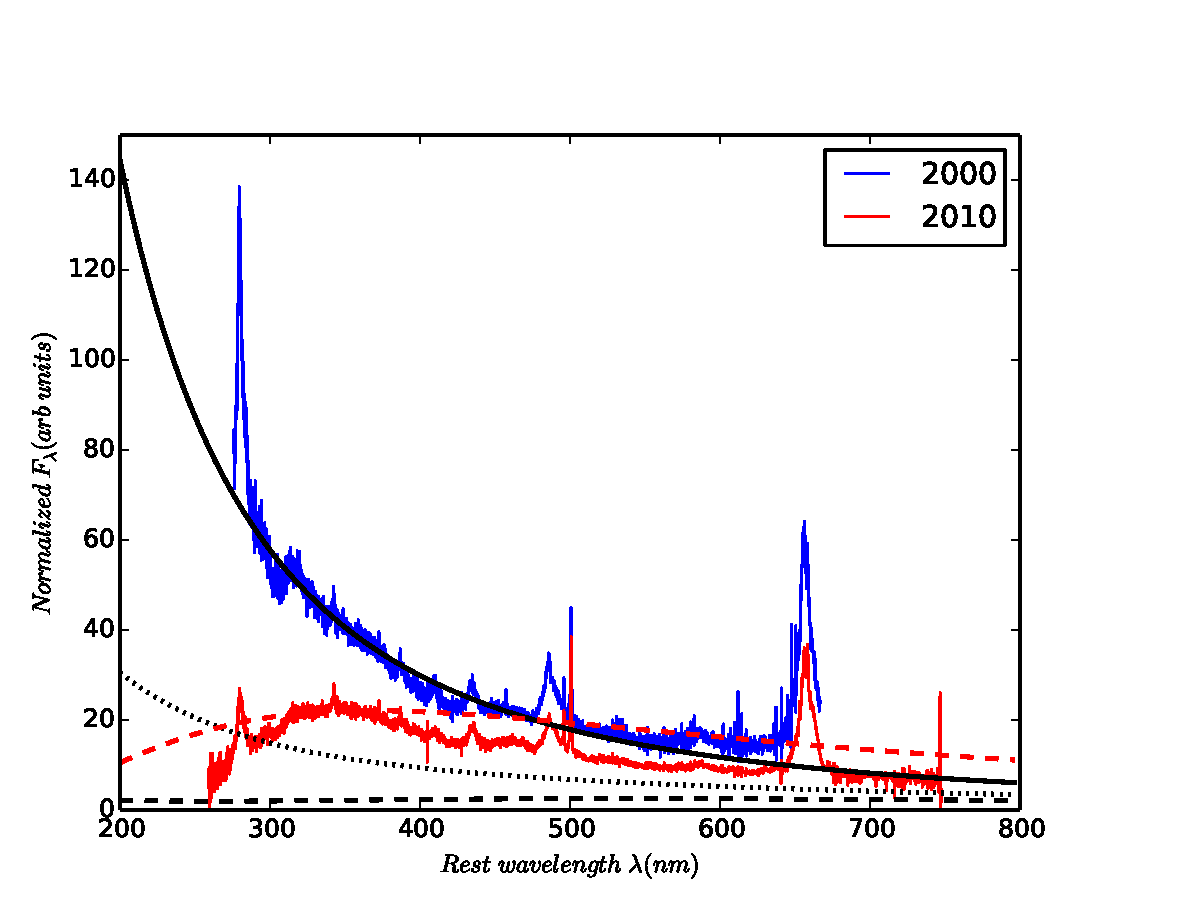
\includegraphics[width=12.00cm, height=10.0cm, trim=0.3cm 0.0cm 2.0cm 0.0cm, clip]
  {../plots/models/mcd_gap_v3_3_b1.pdf}
  \caption[]{
J1100-0053 data (blue line 2000 spectrum; red line 2010 spectrum) and 4
models. Solid black line shows non-zero torque at ISCO
\citep[following] []{Afshordi_Paczynski2003}; dotted and dashed black
lines show temperature suppression inside $r_{\rm alt} = 225 r_{\rm
g}$, such that the spectral flux is $f_{\rm dep} = $ 0.2 or 0.01
(respectively) compared to a zero torque model; dashed red line shows
zero flux inside $r_{\rm alt} = 80 r_{\rm g}$ and arbitrary
normalization to match peak of 2010 spectrum. Note the poor fit due to
the intrinsic width of the thermal peak.
  }
  \label{fig:disk_suppression}
\end{figure*}
Can J1100-0053 switch states from a thin disk quasar to an ADAF at small
radii with the thin disk surviving at large radii?  Assuming the
transition happens due to an instability on the thermal timescale of
the disk, then at large radii the thermal timescale is
\begin{equation}
    t_{\rm th} \sim 14 \; {\rm years} \; \left(\frac{\alpha}{0.03}\right)^{-1}
                                                \left(\frac{r}{225r_{g}}\right)^{3/2} 
                                                        \frac{r_{g}}{c}
\end{equation} 
and is too long given the observations. However, if the viscosity
parameter $\alpha$ increases to $\alpha \approx 0.3$, as suggested by
\citet{King2007}, then the thermal timescale is $t_{\rm th} \sim 1.4$
year and the front timescale is
\begin{equation}
    t_{\rm front}  \sim  10 \; {\rm years} \left(\frac{h/r}{0.05}\right)^{-1}
                                                           \left(\frac{\alpha}{0.3}\right)^{-1}  
                                                           \left(\frac{r}{225r_{g}}\right)^{3/2}  
                                                           \frac{r_{g}}{c}
\label{eqn:t_front}
\end{equation}
which is plausible, if there exists a very viscous disk and the effect
propagates outwards on a timescale of $\leq 10$ years from the inner
disk. This would suppress the UV/X-ray emission from the RIAF (down by
a few orders of magnitude from the intensity expected from a thin disk
intensity) and explain the broadline behaviour.  ADAF spectra are flat
in $\nu L_{\nu}$ \citet{Narayan1998, Abramowicz2002, Abramowicz2013},
and convective ADAFs rise towards X-ray energies. ADAFs exist at lower
luminosity, where $\epsilon \sim 0.005$ for $L=\epsilon \dot{M}
c^{2}$, lower than the fiducial $\epsilon \sim 0.1$ for a classic thin
disk luminosity.

%sf: many edits in 2 para below
However, suppressing the flux from the inner disk radii ($\lesssim 225 r_{g}$)
in the low temperature thin disk model \citep{Narayan1997, Gammie1999,
Agol_Krolik2000, Afshordi_Paczynski2003, Ford2018}, by a factor of
$20$ would still not describe the 2010 spectrum. To restore the thin disk
spectrum by 2016, the disk change has to propagate back inwards, most
of the way to the ISCO and therefore $t_{\rm front}$ needs to be
shorter. This requires $h/r$ to be larger in
Equation~\label{eqn:t_front} above, by a factor of $\sim 2$.

It is unclear what physical processes would trigger the change of
state to an ADAF and then cool back down to a thin disk. However, more
of an issue is that supressing the MCD temperature profile inside a
radius of $r_{alt} = 225 r_{g}$ leads to a collapse in the total
flux compared to unperturbed disk. We show some example cases
in~\ref{fig:disk_suppression}. Clearly, these scenarios are difficult
to reconcile with our data.

\smallskip \smallskip
\noindent
\textbf{\textsc{Model `B': Propagating of a Cooling Front: }}
An alternative model connected to the accretion disk is that a
\emph{cooling} front propagates through the thin disk.  In order to
reproduce the steep fall at $\lambda \leq 200$nm in the 2010 spectrum,
a cool phase leads to absorption at short wavelengths.

Initially a modestly fat disk ($h/r \sim 0.2$) with a modest $\alpha$,
cools from the ISCO and propagates outward in a cooling front,
collapsing the disk. As the hot disk ($\sim 10^{5-6}$K) cools, it
fragments into cooler clumps around $\sim 10^{4}$K \citep[see e.g.,
][]{McCourt2016}.  The main coolants are resonance lines in carbon and
oxygen \citep[see e.g., Fig. 18 in ][]{Sutherland_Dopita1993} The
ionization energies for carbon and carbon are 11.26 and 13.61 eV,
respectively, i.e., $\sim 100$nm, and hence at wavelengths $<100$nm
the disk opacity will increase dramatically in an edge. %sf: edits below
However, the
gas in the disk is both pressure, turbulent and Doppler broadened, so
these ionization edges will manifest around 100nm with decreasing
opacity to shorter wavelengths as
\begin{equation}
  \kappa \propto \rho T^{-1/2} \nu^{-3}
\end{equation}
for Kramers' opacities. This implies $\kappa \propto \lambda^{3}$
at increasing wavelengths up to the ionization edge around $100$nm.
These features will be blurred (by the broadening) and the ionization
edges due to the C and O resonance lines in the cool phase of this
disk will be span $50-200$nm, depressing the flux at these energies.

The 2010 spectrum in this model comes from a cooler disk plus the
increased opacity at short wavelengths in the cooler phase. Heating
occurs from the outside in, explaining the 2016 spectrum and
asymmetric recovery in photometry.  Since the
optical continuum has been rising again since mid-2016, this leads to
a prediction of a rise in hydrogen emission line flux in the next few
months (2018). The infrared flux returns in 2021. 


\begin{figure}[h]
  \centering
  %% trim=l b r t 
  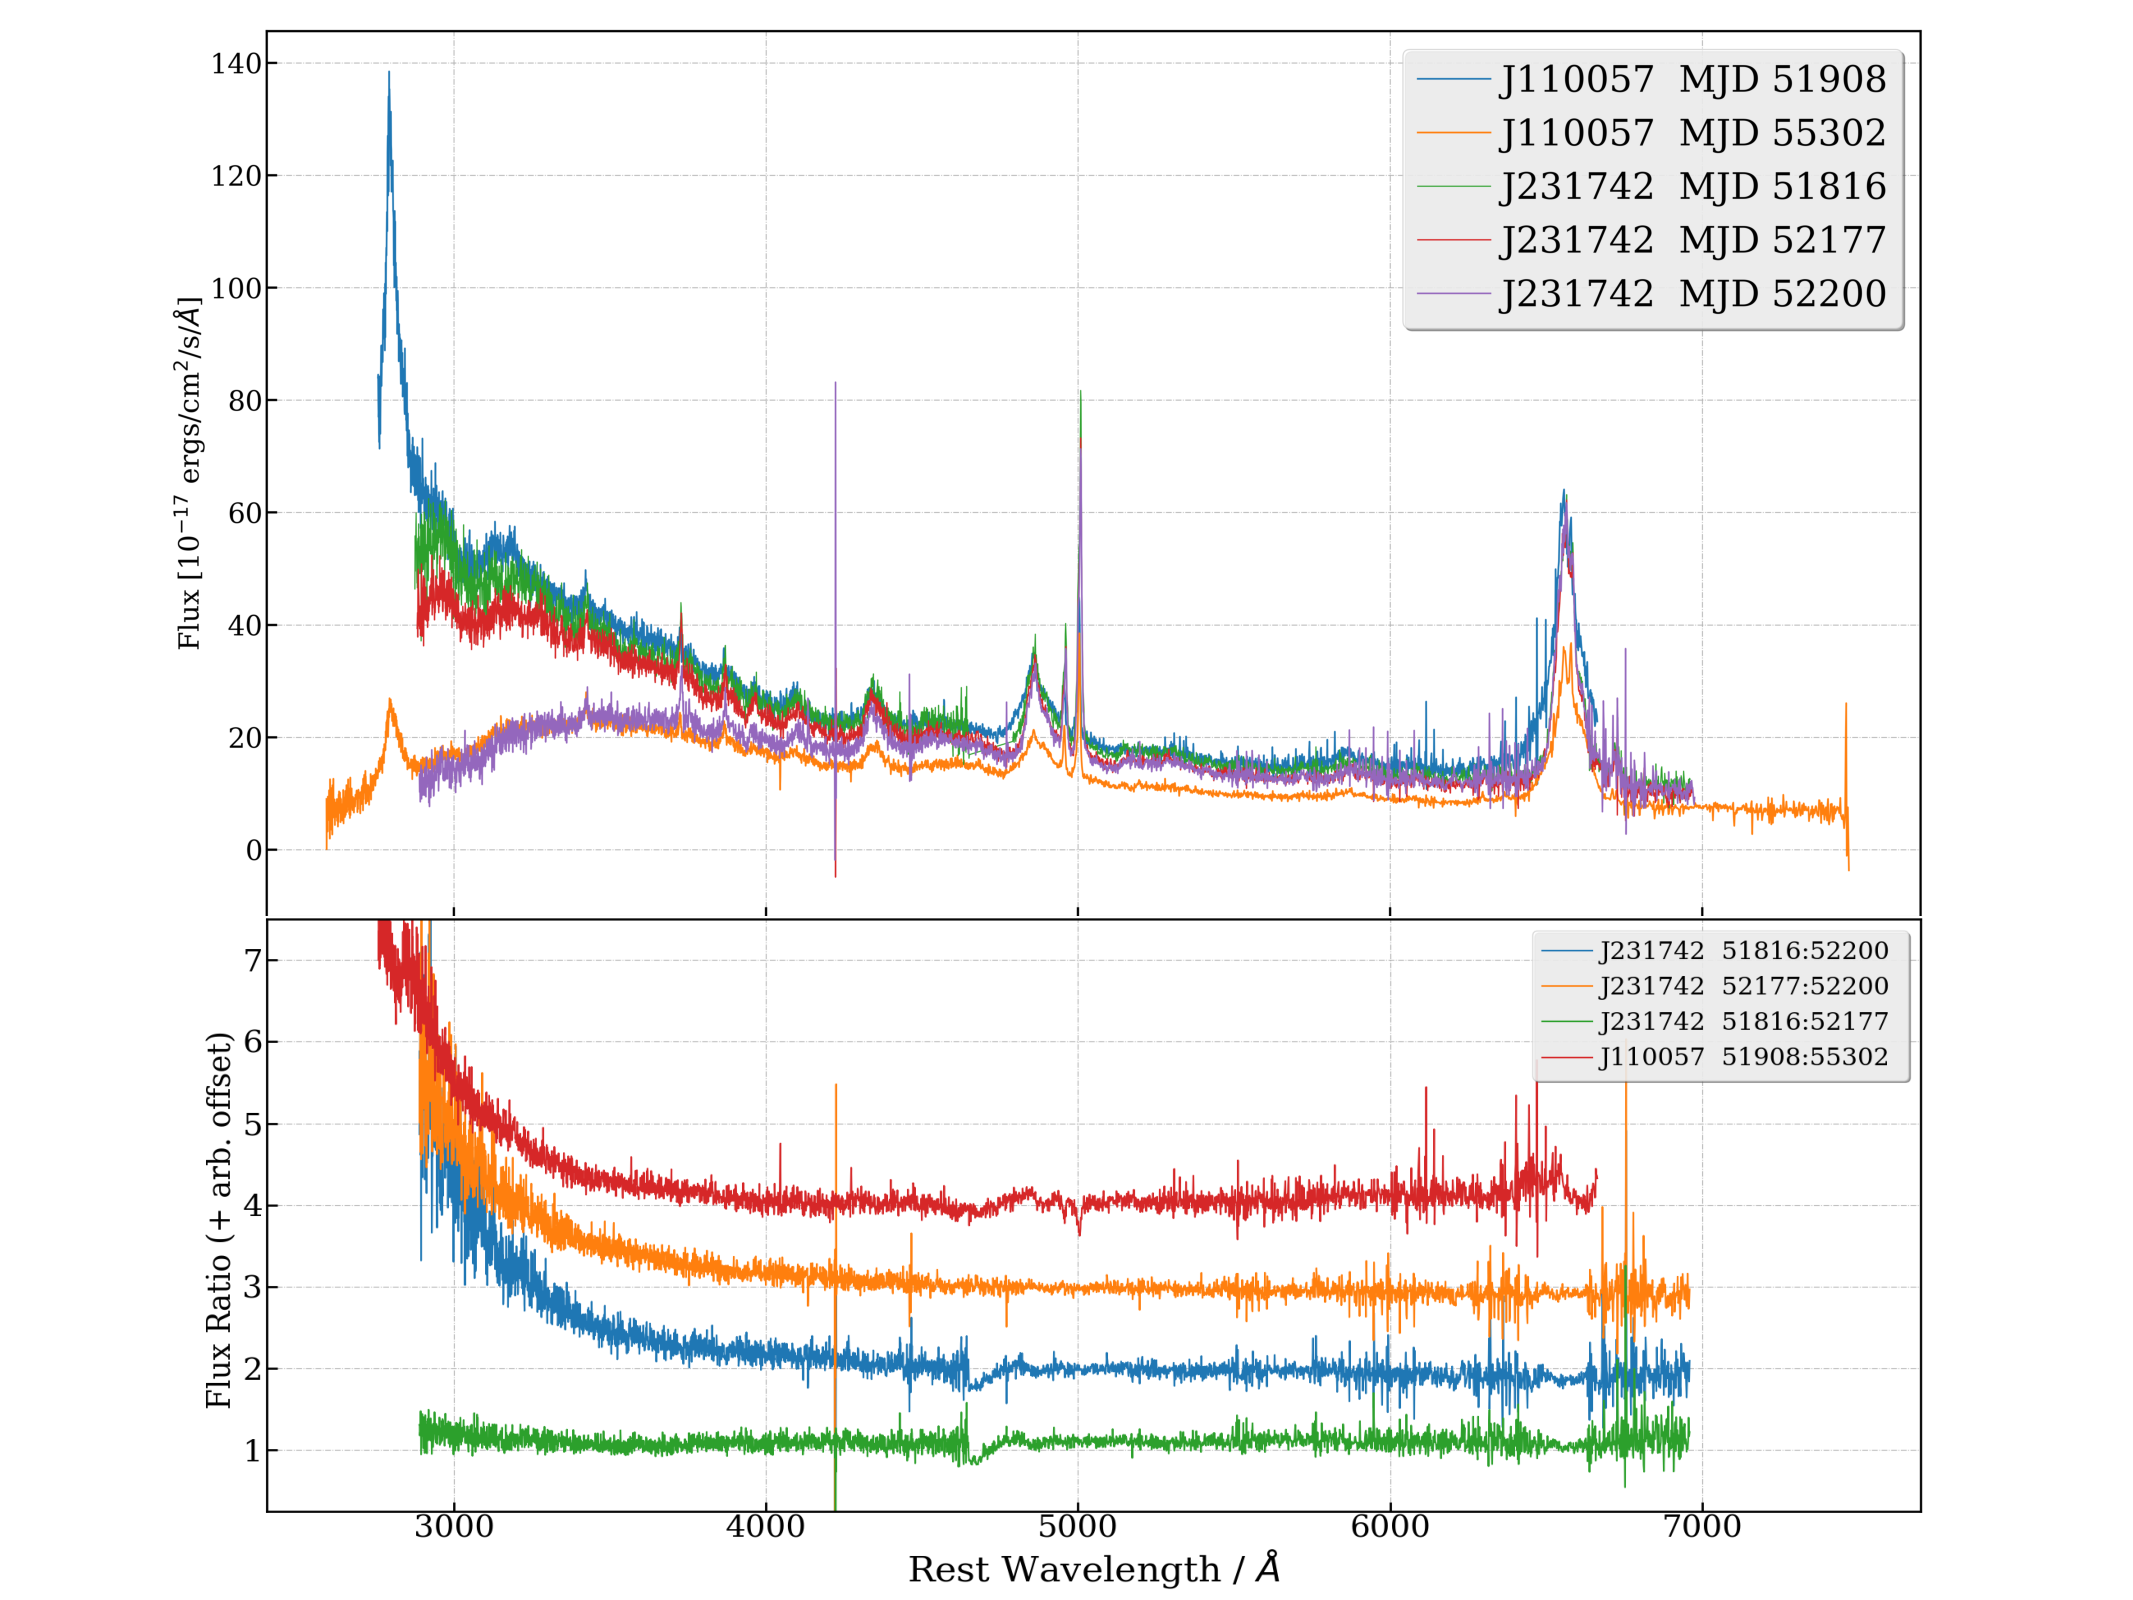
\includegraphics[width=16.00cm, height=12.0cm, trim=0.3cm 0.0cm 2.0cm 0.0cm, clip]
  {../plots/spectra/J110057_vs_Guo_both_20171115.pdf}
  \caption[]{ {\it Top::} The five SDSS/BOSS spectra of J2317+0005 and
    J1100-0053.  The striking similarity between the two spectra downturned in
    the blue can be seen.  {\it Bottom::} The ratio of the different epoch
    spectra.}
  \label{fig:J1100-0053_vs_Guo}
\end{figure}
\section*{Comparison with SDSS J2317+0005 from Guo et al. 2016}
Figure~1 of Guo et al. (2016) shows a UV collapse in the quasar SDSS
J231742.60+000535.1 (hereafter J2317+0005, with redshift $z=0.32$),
similar to that of J1100-0053. In Figure~\ref{fig:J1100-0053_vs_Guo} we show
the five SDSS/BOSS spectra from J1100-0053 and J2317+0005 (top panel),
and their ratios (bottom panel).  The collapse in J2317+0005 happens
in 23 days \citep[Figure 2 of ][]{Guo2016}; this object was observed
by SDSS on MJD 52177 (normal) and then on MJD 52200. In the second
epoch spectrum, there is a drop of 1.2 mag in the $u$-band and 0.5mag
in $g$-band. The $r,i,z$-bands are all consistent with the earlier
observation. J2317+0005 is observed with SDSS $\sim$a year later and
$(u,g,r,i,z)$ are all consistent with the earlier MJD 52177
spectrum. XMM-Newton spectra straddle this time period, from 2001 June
03 to 2001 November 28. Both X-ray spectra are consistent with no neutral
absorption in the rest-frame. This implies the sightline is clear on
both of those dates.  \citet{Guo2016} also find that the IR does not
significantly change and that the broad lines are consistent with
being constant over time.

\citet{Guo2016} discuss two scenarios to explain this behaviour: {\it
(i)} an inner accretion disk change and {\it (ii)} an eclipse by an
optically thick cloud. \citet{Guo2016} note that in principle both
models could explain the observation. In the inner accretion disk
scenario, turning off the disk at $r < 60 r_{\rm g}$ would explain the
J2317+0005 spectra, though the detailed MCD fit is far from ideal, in
much the same manner as for J11057. However, \citet{Guo2016} find this
explanation unconvincing since ``quasars are not observed to flicker
like this typically''.  The second scenario is favoured based on the
initial optical spectrum (23 days before the $u$-band dip) and the
2001 November X-ray spectrum (45 days after the $u$-band dip).  For
the reasons given above for J1100-0053, and in particular with our
infrared light curve data, we suggest $\approx$45 days is too short
for an obscuration event, and hence suggest that the same initial
cause (model B above: a cooling front propagating from the inner
accretion disk) explains \emph{both} the \citet{Guo2016} spectrum and
our 2010 spectrum. In the case of the \citet{Guo2016} source, the fact
that the IR and broad lines are unchanged implies that the temporary
disk dimming is very short-lived. Therefore, in the case of
\citet{Guo2016}, the restoring heating front must propagate outwards
from the inner disk. This is unlike J1100-0053 (model B above), where the
restoring heating front must propagate inwards from the outer disk in
order to explain the restoration of {\it g}-band before {\it u}-band
and the long-term supression of broad lines and IR.


\section*{Acknowledgements}
NPR acknowledges support from the STFC and the Ernest Ruther- ford
Fellowship scheme.  KESF \& BM are supported by NSF PAARE
AST-1153335. KESF \& BM thank CalTech/JPL for support during
sabbatical.  MF acknowledges support from NSF grants AST-1518308,
AST-1749235, AST-1413600 and NASA grant 16-ADAP16-0232.

Funding for SDSS-III has been provided by the Alfred P. Sloan
Foundation, the Participating Institutions, the National Science
Foundation, and the U.S. Department of Energy Office of Science. The
SDSS-III web site is
\href{http://www.sdss3.org/}{http://www.sdss3.org/}.

SDSS-III is managed by the Astrophysical Research Consortium for the
Participating Institutions of the SDSS-III Collaboration including the
University of Arizona, the Brazilian Participation Group, Brookhaven
National Laboratory, Carnegie Mellon University, University of
Florida, the French Participation Group, the German Participation
Group, Harvard University, the Instituto de Astrofisica de Canarias,
the Michigan State/Notre Dame/JINA Participation Group, Johns Hopkins
University, Lawrence Berkeley National Laboratory, Max Planck
Institute for Astrophysics, Max Planck Institute for Extraterrestrial
Physics, New Mexico State University, New York University, Ohio State
University, Pennsylvania State University, University of Portsmouth,
Princeton University, the Spanish Participation Group, University of
Tokyo, University of Utah, Vanderbilt University, University of
Virginia, University of Washington, and Yale University.

This publication makes use of data products from the Wide-field
Infrared Survey Explorer, which is a joint project of the University
of California, Los Angeles, and the Jet Propulsion
Laboratory/California Institute of Technology, and NEOWISE, which is a
project of the Jet Propulsion Laboratory/California Institute of
Technology. WISE and NEOWISE are funded by the National Aeronautics
and Space Administration.

This research has made use of the NASA/IPAC Extragalactic Database
(NED) which is operated by the Jet Propulsion Laboratory, California
Institute of Technology, under contract with the National Aeronautics
and Space Administration.



\bibliographystyle{mn2e}
\bibliography{/cos_pc19a_npr/LaTeX/tester_mnras}


\end{document}